% Provenance (never printed): see sources/outline_sources.md (Year 1: optical
% mineralogy with the polarising microscope; Michel-Levy chart). Interference
% colours in figdata/bachelor-1/michel_levy.py from the CIE 1931 colour-matching
% functions and illuminant D65 (data/derived/bachelor-1-cie*.csv); exercise and
% problem values in the Book 3 scratch calculator calc/ch08.py.
\chapter{Optische mineralogie}\label{ch:b1:optical-mineralogy}

Tussen \omterm{def:b1:field-lab-methods-1:microscope}{gekruiste polarisatoren} licht een \omterm{def:b1:field-lab-methods-1:thin-section}{dunne slijpplaat} van gabbro op als glas-in-lood. Lange grijze en witte latten,
gestreept als een barcode, kruisen het beeld; daartussen gloeien korrels blauw, geel en magenta; enkele blijven zwart, wat de
hoek ook is. Elk van deze effecten heeft een oorzaak die berekend kan worden, en elk vertelt welk \omterm{def:b1:rock-forming-minerals:mineral}{mineraal} er zit. Dit hoofdstuk
legt uit hoe licht een kristal doorloopt, waarom een \omterm{def:b1:rock-forming-minerals:mineral}{mineraal} tussen \omterm{def:b1:field-lab-methods-1:microscope}{gekruiste polarisatoren} gekleurd is, hoe de kleur een eigenschap
van het \omterm{def:b1:rock-forming-minerals:mineral}{mineraal} meet, en hoe een petroloog de korrels van een \omterm{def:b1:field-lab-methods-1:thin-section}{slijpplaat} benoemt met niets dan een microscoop. Het eindigt met een
onbekende \omterm{def:b1:field-lab-methods-1:thin-section}{slijpplaat}, waarvan de mineralen en de \omterm{def:b1:cross-sections:thickness}{ware dikte} uit wat zij toont worden afgeleid.

\begin{recall}
Een \omterm{def:b1:field-lab-methods-1:thin-section}{dunne slijpplaat} is een plakje gesteente van ongeveer \qty{30}{\micro m} dik op een glazen plaatje; de \omterm{def:b1:field-lab-methods-1:microscope}{polariserende microscoop}
bekijkt haar in \omterm{def:b1:field-lab-methods-1:microscope}{vlakgepolariseerd licht} (één polarisator) en tussen \omterm{def:b1:field-lab-methods-1:microscope}{gekruiste polarisatoren} (\cref{ch:b1:field-lab-methods-1}). De
brekingsindex $n$ van een medium is de verhouding van de lichtsnelheid in vacuüm tot die in het medium, en breking op een grensvlak
gehoorzaamt aan de wet van Snellius $n_1\sin i_1 = n_2\sin i_2$ (natuurkunde, eerste jaar universiteit). Licht is een transversale
golf; een polarisator laat alleen de component van het elektrische veld langs zijn richting door, zodat een analysator onder de hoek
$\alpha$ ten opzichte ervan de fractie $\cos^2\alpha$ van de intensiteit doorlaat (de wet van Malus, natuurkunde).
\end{recall}

\section{Licht in kristallen}

In een glas, een vloeistof of een kubisch kristal reist licht met dezelfde snelheid in elke richting en ongeacht zijn trillingsrichting.
In de meeste mineralen is dat niet zo: de rangschikking van de atomen verschilt langs verschillende richtingen, en dus ook de reactie van de
elektronen op het elektrische veld van de golf.

\begin{definition}[Isotrope en anisotrope mineralen]\label{def:b1:optical-mineralogy:anisotropic}
Een \omterm{def:b1:rock-forming-minerals:mineral}{mineraal} is een \emph{isotroop mineraal}\index{isotroop mineraal} wanneer zijn brekingsindex voor elke richting van voortplanting en
van trilling van het licht dezelfde is; kubische mineralen (\omterm{def:b1:rock-forming-minerals:groups}{granaat}, haliet, spinel) en glazen zijn isotroop. Het is een
\emph{anisotroop mineraal}\index{anisotroop mineraal} wanneer zijn brekingsindex van de trillingsrichting afhangt; alle mineralen van de
andere kristalstelsels zijn anisotroop.
\end{definition}
Een plaatje dat uit een anisotroop kristal is gesneden, laat het licht niet als één golf door. Wij aanvaarden het volgende resultaat van de
kristaloptica (natuurkunde, tweede jaar universiteit): voor een gegeven voortplantingsrichting laat een plaatje van een \omterm{def:b1:optical-mineralogy:anisotropic}{anisotroop mineraal}
twee golven door die in twee loodrechte richtingen trillen die in het plaatje vastliggen, haar \emph{trillingsrichtingen}, en met twee
verschillende brekingsindices $n_1$ en $n_2$ reizen. Licht dat in één van deze richtingen trilt, gaat ongewijzigd in polarisatie door het
plaatje; licht dat in een andere richting trilt, wordt in zijn twee componenten langs hen gesplitst. De twee indices hangen af van de
voortplantingsrichting, en er zijn bijzondere richtingen waarin zij gelijk zijn.

\begin{definition}[Optische as, eenassige en tweeassige mineralen]\label{def:b1:optical-mineralogy:optic-axis}
Een \emph{optische as}\index{optische as} van een \omterm{def:b1:optical-mineralogy:anisotropic}{anisotroop mineraal} is een voortplantingsrichting waarlangs het licht met één
enkele brekingsindex reist, ongeacht zijn trillingsrichting, zoals in een isotroop medium. Een \omterm{def:b1:rock-forming-minerals:mineral}{mineraal} is \emph{eenassig}\index{eenassig}
wanneer het één optische as heeft (mineralen van het trigonale, tetragonale en hexagonale stelsel, zoals kwarts en calciet) en
\emph{tweeassig}\index{tweeassig} wanneer het er twee heeft (rombische, monokliene en trikliene mineralen, zoals \omterm{def:b1:rock-forming-minerals:groups}{olivijn}, pyroxenen,
amfibolen, \omterm{def:b1:rock-forming-minerals:groups}{micas} en veldspaten).
\end{definition}

De meetkunde wordt samengevat door een oppervlak, de indicatrix: een ellipsoïde waarvan de straal in elke richting de brekingsindex is voor
licht dat in die richting trilt. De doorsnede van de ellipsoïde loodrecht op de voortplantingsrichting is een ellips waarvan de assen de twee
trillingsrichtingen zijn en waarvan de halve assen $n_1$ en $n_2$ zijn. Voor een \omterm{def:b1:optical-mineralogy:optic-axis}{eenassig} \omterm{def:b1:rock-forming-minerals:mineral}{mineraal} is de ellipsoïde een omwentelingslichaam om
de \omterm{def:b1:optical-mineralogy:optic-axis}{optische as}, met twee hoofdindices $n_\omega$ en $n_\varepsilon$: kwarts heeft $n_\omega = 1.544$ en $n_\varepsilon = 1.553$, calciet
$1.658$ en $1.486$.
% ledger: hom:quartz-optics, hom:calcite-optics
Een \omterm{def:b1:optical-mineralogy:optic-axis}{tweeassig} \omterm{def:b1:rock-forming-minerals:mineral}{mineraal} heeft drie hoofdindices $n_\alpha < n_\beta < n_\gamma$ en twee cirkelvormige doorsneden, loodrecht op zijn twee optische
assen: forsteriet heeft $1.635$, $1.651$ en $1.670$.
% ledger: hom:forsterite-optics

\begin{definition}[Dubbelbreking (van een mineraal)]\label{def:b1:optical-mineralogy:birefringence}
De \emph{dubbelbreking}\index{dubbelbreking (van een mineraal)} van een \omterm{def:b1:rock-forming-minerals:mineral}{mineraal} is het verschil $\delta = n_{\max} - n_{\min}$ tussen zijn grootste en
kleinste hoofdbrekingsindices: $n_\varepsilon - n_\omega$ in absolute waarde voor een \omterm{def:b1:optical-mineralogy:optic-axis}{eenassig} \omterm{def:b1:rock-forming-minerals:mineral}{mineraal}, $n_\gamma - n_\alpha$ voor een \omterm{def:b1:optical-mineralogy:optic-axis}{tweeassig}.
In een korrel die in een andere richting is gesneden, ligt het verschil $|n_1 - n_2|$ tussen 0 (een doorsnede loodrecht op een \omterm{def:b1:optical-mineralogy:optic-axis}{optische as}) en
$\delta$ (een doorsnede die de richtingen van $n_{\max}$ en $n_{\min}$ bevat).
\end{definition}

De \omterm{def:b1:optical-mineralogy:birefringence}{dubbelbreking} is een eigenschap van het \omterm{def:b1:rock-forming-minerals:mineral}{mineraal}, zoals zijn dichtheid: kwarts \num{0.009}, calciet \num{0.172}, forsteriet \num{0.035},
fayaliet \num{0.052}. Een \omterm{def:b1:field-lab-methods-1:thin-section}{slijpplaat} snijdt de korrels van een \omterm{def:b1:rock-forming-minerals:mineral}{mineraal} in alle oriëntaties, dus tonen zijn korrels elke waarde van 0 tot $\delta$;
alleen de hoogste is kenmerkend.
% ledger: hom:quartz-optics, hom:calcite-optics, hom:forsterite-optics, hom:fayalite-optics

\section{Waarnemingen in vlakgepolariseerd licht}

Met alleen de onderste polarisator toont de microscoop de vorm van de korrels, hun kleur, hun splijtingen en hun \omterm{def:b1:optical-mineralogy:relief}{reliëf}.

\begin{definition}[Pleochroïsme]\label{def:b1:optical-mineralogy:pleochroism}
Een \omterm{def:b1:rock-forming-minerals:mineral}{mineraal} is \emph{pleochroïsch}\index{pleochroïsme} wanneer zijn kleur, gezien in \omterm{def:b1:field-lab-methods-1:microscope}{vlakgepolariseerd licht}, verandert als de tafel
wordt gedraaid; het \emph{pleochroïsme} is die verandering. Zij ontstaat doordat de absorptie van licht afhangt van zijn trillingsrichting
in het kristal.
\end{definition}

Biotiet is het leerboekvoorbeeld: een korrel die dwars op haar splijting is gesneden, gaat van lichtgeel-bruin naar donkerbruin wanneer zij
draait, het donkerst wanneer de splijtsporen langs de polarisator liggen. Hoornblende verandert van geel naar groen. De meeste andere
gesteentevormende silicaten (kwarts, veldspaten, \omterm{def:b1:rock-forming-minerals:groups}{olivijn}, diopsied, muscoviet) zijn kleurloos in \omterm{def:b1:field-lab-methods-1:thin-section}{slijpplaat}, en hun kleurloze korrels worden
op andere manieren onderscheiden.
% ledger: hom:biotite-optics, hom:hornblende-optics, hom:muscovite-optics, hom:diopside-optics, hom:forsterite-optics

\begin{definition}[Reliëf, Becke-lijn]\label{def:b1:optical-mineralogy:relief}
Het \emph{reliëf}\index{reliëf (optisch)} van een korrel in \omterm{def:b1:field-lab-methods-1:thin-section}{slijpplaat} is hoe sterk haar omtrek, scheuren en oppervlak afsteken tegen het
insluitmiddel; het is hoog wanneer de brekingsindices van de korrel en van het middel sterk verschillen, laag wanneer zij dicht bij elkaar liggen.
De \emph{Becke-lijn}\index{Becke-lijn} is de dunne heldere lijn die een korrel omzoomt waarvan de index afwijkt van die van haar omgeving, wanneer
de microscoop enigszins uit scherp staat.
\end{definition}

\begin{proposition}[Reliëf en brekingsindex]\label{prop:b1:optical-mineralogy:relief}
Een straal die onder inval $i$ een grensvlak snijdt tussen een insluitmiddel met index $n_m$ en een korrel met index $n$ dicht bij $n_m$, wordt
afgebogen over
\[
  \varepsilon \approx \frac{|n - n_m|}{n_m}\,\tan i
\]
(in radialen), tot de eerste \omterm{def:b1:optical-mineralogy:interference-colour}{orde} in $(n - n_m)/n_m$. De afbuigingen aan de schuine randen van een korrel, en dus haar \omterm{def:b1:optical-mineralogy:relief}{reliëf}, groeien evenredig
met $|n - n_m|$.
\end{proposition}

\begin{proof}
De wet van Snellius geeft $n_m \sin i = n \sin r$. Schrijf $n = n_m(1 + \eta)$ met $\eta$ klein en $r = i - \varepsilon$ met $\varepsilon$ klein. Dan
geldt $\sin i = (1 + \eta)(\sin i - \varepsilon\cos i) + O(\eta^2, \varepsilon^2)$, dus $\eta \sin i = \varepsilon\cos i$ tot de eerste \omterm{def:b1:optical-mineralogy:interference-colour}{orde}, dat wil
zeggen $\varepsilon = \eta\tan i$, met $|\eta| = |n - n_m|/n_m$.
\end{proof}

Een \omterm{def:b1:field-lab-methods-1:thin-section}{slijpplaat} is gemonteerd in een hars met een index van ongeveer $1.54$.
% ledger: jaic:epoxy-ri
Kwarts ($1.544$--$1.553$) en de veldspaten ($1.52$--$1.59$) zijn er bijna onzichtbaar in: laag \omterm{def:b1:optical-mineralogy:relief}{reliëf}, de korrelgrenzen moeilijk te zien.
\omterm{def:b1:rock-forming-minerals:groups}{Olivijn} ($1.64$--$1.88$), pyroxenen en amfibolen steken af met donkere randen en een ruw ogend oppervlak: hoog \omterm{def:b1:optical-mineralogy:relief}{reliëf}. \omterm{def:b1:rock-forming-minerals:groups}{Granaat} ($1.83$) lijkt bijna
zwartomrand. Calciet, waarvan de index van $1.486$ tot $1.658$ loopt met de trillingsrichting, verandert van \omterm{def:b1:optical-mineralogy:relief}{reliëf} wanneer de tafel draait, een effect dat
fonkelen heet.
% ledger: hom:quartz-optics, hom:albite-optics, hom:anorthite-optics, hom:orthoclase-optics, hom:forsterite-optics, hom:fayalite-optics, hom:almandine-optics, hom:calcite-optics
Het \omterm{def:b1:optical-mineralogy:relief}{reliëf} vertelt alleen hoe ver $n$ van $n_m$ af ligt, niet aan welke kant; de \omterm{def:b1:optical-mineralogy:relief}{Becke-lijn} vertelt de kant.

\begin{method}[De Becke-lijntest]\label{met:b1:optical-mineralogy:becke}
Stel scherp op de rand van een korrel in \omterm{def:b1:field-lab-methods-1:microscope}{vlakgepolariseerd licht}, sluit het diafragma een weinig, en trek de scherpstelling iets aan (beweeg het objectief
weg van de doorsnede). De heldere \omterm{def:b1:optical-mineralogy:relief}{Becke-lijn} beweegt het middel met de hogere brekingsindex in: beweegt zij de korrel in, dan heeft de korrel de hogere
index (positief \omterm{def:b1:optical-mineralogy:relief}{reliëf}); beweegt zij naar buiten, naar het insluitmiddel of de buurkorrel, dan heeft de korrel de lagere index (negatief \omterm{def:b1:optical-mineralogy:relief}{reliëf}).
\end{method}

De methode werkt omdat een korrelgrens nooit precies verticaal is: bij een schuine grens wordt het licht naar de kant van de hogere index gebroken,
en voorbij de grenshoek wordt het op die kant totaal teruggekaatst, zodat het licht dat de grens kruist boven het materiaal met de hogere index
geconcentreerd wordt. Het scherpstellen op een vlak boven de doorsnede kijkt naar dat geconcentreerde licht, dat binnen het materiaal met de hogere index ligt.

\section{Tussen gekruiste polarisatoren}

Met de analysator ingeschoven, loodrecht op de polarisator, is een isotrope korrel in elke stand zwart: het licht bereikt haar trillend langs de polarisator
en verlaat haar zo trillend, en de analysator houdt het volledig tegen. Een anisotrope korrel is over het algemeen helder en gekleurd. De reden is de
vertraging tussen haar twee golven.

\begin{definition}[Retardatie (in een kristalplaatje)]\label{def:b1:optical-mineralogy:retardation}
De \emph{retardatie}\index{retardatie (in een kristalplaatje)} $\Delta$ van een plaatje van een \omterm{def:b1:optical-mineralogy:anisotropic}{anisotroop mineraal} is het verschil tussen de optische
weglengten van haar twee golven bij het verlaten van het plaatje, waarbij de langzamere golf achterloopt op de snellere.
\end{definition}

\begin{proposition}[Retardatie en dubbelbreking]\label{prop:b1:optical-mineralogy:retardation}
Een plaatje met dikte $d$ waarvan de twee golven indices $n_1 > n_2$ hebben, heeft de \omterm{def:b1:optical-mineralogy:retardation}{retardatie}
\[
  \Delta = d\,(n_1 - n_2),
\]
en haar twee golven verlaten het met een faseverschil $\varphi = 2\pi\Delta/\lambda$ voor licht met golflengte $\lambda$ in vacuüm. In een \omterm{def:b1:field-lab-methods-1:thin-section}{dunne slijpplaat}
is de grootste \omterm{def:b1:optical-mineralogy:retardation}{retardatie} die korrels van één \omterm{def:b1:rock-forming-minerals:mineral}{mineraal} tonen $d\,\delta$.
\end{proposition}

\begin{proof}
Een golf die een dikte $d$ doorloopt met snelheid $c/n$, doet er $nd/c$ over; haar optische weglengte, de afstand die licht in vacuüm in die tijd zou afleggen,
is $nd$. De twee golven treden samen binnen; bij het verlaten loopt de langzamere achter met $n_1 d - n_2 d = d(n_1 - n_2)$, een vertraging die de
breuk $\Delta/\lambda$ van een periode is, dat wil zeggen een fase $2\pi\Delta/\lambda$. De grootste waarde van $n_1 - n_2$ over alle oriëntaties is $\delta$
(\cref{def:b1:optical-mineralogy:birefringence}).
\end{proof}

Een kwartskorrel van de gunstigste oriëntatie in een doorsnede van \qty{30}{\micro m} dik heeft $\Delta = \qty{30000}{nm}\times0.009 =
\qty{270}{nm}$; een calcietkorrel $\qty{30000}{nm}\times0.172 = \qty{5160}{nm}$.

\begin{omfigure}
\begin{tikzpicture}[x=1cm, y=1cm, >={Stealth},
  sub/.style={align=center, font=\small, text width=4.2cm}]
% (a) the polariser
\begin{scope}
  \draw[gray!60] (-1.4,0) -- (1.4,0) (0,-1.4) -- (0,1.4);
  \node[gray, font=\scriptsize] at (1.55,-0.2) {E};
  \node[gray, font=\scriptsize] at (0.2,1.55) {N};
  \draw[very thick, omDef, <->] (-1.2,0) -- (1.2,0);
  \node[omDef, font=\scriptsize, above] at (0.75,0.05) {$E_0$};
  \node[sub] at (0,-2.1) {(a) na de polarisator:\\ trilling oost--west};
\end{scope}
% (b) inside the plate
\begin{scope}[shift={(5.0,0)}]
  \draw[gray!60] (-1.4,0) -- (1.4,0) (0,-1.4) -- (0,1.4);
  \draw[omThm, thick] (-1.35*0.866,-1.35*0.5) -- (1.35*0.866,1.35*0.5);
  \draw[omThm, thick] (1.35*0.5,-1.35*0.866) -- (-1.35*0.5,1.35*0.866);
  \node[omThm, font=\scriptsize] at (1.42,0.95) {1};
  \node[omThm, font=\scriptsize] at (-0.85,1.32) {2};
  \draw[very thick, omDef, ->] (0,0) -- (1.2,0);
  \draw[omProp, very thick, ->] (0,0) -- (1.2*0.866*0.866,1.2*0.866*0.5);
  \draw[omProp, very thick, ->] (0,0) -- (1.2*0.5*0.5,-1.2*0.5*0.866);
  \draw[densely dotted] (1.2,0) -- (1.2*0.866*0.866,1.2*0.866*0.5) (1.2,0) -- (1.2*0.5*0.5,-1.2*0.5*0.866);
  \draw (0.55,0) arc[start angle=0, end angle=30, radius=0.55];
  \node[font=\scriptsize] at (0.75,0.17) {$\theta$};
  \node[omProp, font=\scriptsize] at (0.45,1.0) {$E_0\cos\theta$};
  \node[omProp, font=\scriptsize, anchor=east] at (0.1,-0.85) {$E_0\sin\theta$};
  \node[sub] at (0,-2.1) {(b) in het plaatje: twee golven langs\\ de trillingsrichtingen 1 en 2};
\end{scope}
% (c) at the analyser
\begin{scope}[shift={(10.0,0)}]
  \draw[gray!60] (-1.4,0) -- (1.4,0);
  \draw[very thick, omMeth, <->] (0,-1.3) -- (0,1.3);
  \node[omMeth, font=\scriptsize, right] at (0.05,1.2) {analysator};
  \draw[omProp, very thick, ->] (0,0) -- (1.2*0.866*0.866,1.2*0.866*0.5);
  \draw[omProp, very thick, ->] (0,0) -- (1.2*0.5*0.5,-1.2*0.5*0.866);
  \draw[densely dotted] (1.2*0.866*0.866,1.2*0.866*0.5) -- (0,1.2*0.866*0.5)
                        (1.2*0.5*0.5,-1.2*0.5*0.866) -- (0,-1.2*0.5*0.866);
  \draw[omMeth, very thick, ->] (0,0) -- (0,1.2*0.866*0.5);
  \draw[omMeth, very thick, ->] (0,0) -- (0,-1.2*0.5*0.866);
  \node[omMeth, font=\scriptsize, anchor=east] at (-0.08,0.52) {$+E_0\sin\theta\cos\theta$};
  \node[omMeth, font=\scriptsize, anchor=east] at (-0.08,-0.52) {$-E_0\sin\theta\cos\theta$};
  \node[sub] at (0,-2.1) {(c) bij de analysator: elke golf\\ laat haar noord--zuidcomponent door};
\end{scope}
\end{tikzpicture}

{\small Licht door een kristalplaatje tussen \omterm{def:b1:field-lab-methods-1:microscope}{gekruiste polarisatoren}. De polarisator laat de oost--west-trilling door (a); het plaatje splitst die in twee golven
langs haar trillingsrichtingen, onder $\theta$ en $\theta + \ang{90}$ ten opzichte van de polarisator (b); de analysator, noord--zuid, laat de noord--zuidcomponent van
elk door (c). De twee componenten hebben gelijke grootte en tegengestelde tekens: zonder vertraging heffen zij elkaar op, en het plaatje ziet er donker uit; golf 2 loopt
achter golf 1 met de fase $\varphi = 2\pi\Delta/\lambda$, en de som verdwijnt niet meer.}
\end{omfigure}

\begin{theorem}[Intensiteit tussen gekruiste polarisatoren]\label{thm:b1:optical-mineralogy:intensity}
Een plaatje met \omterm{def:b1:optical-mineralogy:retardation}{retardatie} $\Delta$ waarvan de trillingsrichtingen de hoek $\theta$ met de polarisator maken, laat tussen \omterm{def:b1:field-lab-methods-1:microscope}{gekruiste polarisatoren} bij de
golflengte $\lambda$ de intensiteit
\[
  I = I_0\,\sin^2 2\theta\,\sin^2\frac{\pi\Delta}{\lambda},
\]
door, waarin $I_0$ de intensiteit is die de polarisator verlaat.
\end{theorem}

\begin{proof}
Neem de polarisator langs $x$ en de analysator langs $y$, en schrijf het veld dat de polarisator verlaat als het reële deel van $E_0 e^{i\omega t}$ langs $x$, met
$I_0 = E_0^2$ tot op een constante. De trillingsrichting 1 van het plaatje is de eenheidsvector $(\cos\theta, \sin\theta)$, richting 2 is $(-\sin\theta, \cos\theta)$.
Het invallende veld heeft de componenten $E_0\cos\theta$ langs 1 en $-E_0\sin\theta$ langs 2. Het plaatje laat golf 1 ongewijzigd, tot op een gemeenschappelijke
fase, en vertraagt golf 2 met $\varphi = 2\pi\Delta/\lambda$ (\cref{prop:b1:optical-mineralogy:retardation}); in complexe amplituden zijn de golven die het plaatje
verlaten $E_0\cos\theta$ langs 1 en $-E_0\sin\theta\,e^{-i\varphi}$ langs 2. Hun componenten langs $y$ zijn $E_0\cos\theta\sin\theta$ en
$-E_0\sin\theta\cos\theta\,e^{-i\varphi}$; de analysator laat hun som door,
\[
  A = E_0\sin\theta\cos\theta\,(1 - e^{-i\varphi}) .
\]
Omdat $|1 - e^{-i\varphi}|^2 = 2 - 2\cos\varphi = 4\sin^2(\varphi/2)$ en
$\sin\theta\cos\theta = \frac12\sin2\theta$, is de intensiteit
$|A|^2 = E_0^2\,\sin^2 2\theta\,\sin^2(\varphi/2)$, dat is
$I = I_0\sin^2 2\theta\sin^2(\pi\Delta/\lambda)$. Als golf 1 de langzamere is, verandert
$\varphi$ van teken en blijft $I$ onveranderd.
\end{proof}

Het theorema bevat alles wat de microscoop tussen \omterm{def:b1:field-lab-methods-1:microscope}{gekruiste polarisatoren} toont. Zijn eerste factor hangt alleen af van de oriëntatie van de korrel
op de tafel; de tweede alleen van de \omterm{def:b1:optical-mineralogy:retardation}{retardatie} van de korrel en van de kleur van het licht.

\begin{definition}[Uitdovingsstand, uitdovingshoek]\label{def:b1:optical-mineralogy:extinction}
Een anisotrope korrel tussen \omterm{def:b1:field-lab-methods-1:microscope}{gekruiste polarisatoren} staat in een \emph{uitdovingsstand}\index{uitdovingsstand} wanneer zij donker is omdat
haar trillingsrichtingen evenwijdig zijn aan de polarisator en de analysator. De \emph{uitdovingshoek}\index{uitdovingshoek} van een korrel is de hoek
tussen een richting die in haar zichtbaar is (een splijtspoor, een lengterichting, een tweelingvlak) en de dichtstbijzijnde uitdovingsstand, afgelezen op de
geijkte tafel.
\end{definition}

De factor $\sin^2 2\theta$ verdwijnt bij $\theta = 0$, \ang{90}, \ang{180} en \ang{270}: een korrel wordt vier keer per volledige omwenteling van de tafel donker,
en is het helderst halverwege, op \ang{45} van de uitdoving (figuur hieronder). Een korrel met $\Delta = 0$ --- een \omterm{def:b1:optical-mineralogy:anisotropic}{isotroop mineraal}, of een doorsnede
loodrecht op een \omterm{def:b1:optical-mineralogy:optic-axis}{optische as} --- blijft de hele tijd donker. De \omterm{def:b1:optical-mineralogy:extinction}{uitdovingshoek} hangt af van de symmetrie van het kristal: een \omterm{def:b1:rock-forming-minerals:mineral}{mineraal} waarvan de
trillingsrichtingen aan zijn splijtingen gebonden zijn, zoals in rombische mineralen, dooft evenwijdig eraan uit (rechte uitdoving); een monokliene of
trikliene doet dat over het algemeen niet (schuine uitdoving). De grootste \omterm{def:b1:optical-mineralogy:extinction}{uitdovingshoek} tussen de splijtsporen en de langzame trillingsrichting is
ongeveer \ang{38} in diopsied en \ang{15}--\ang{19} in hoornblende, in doorsneden evenwijdig aan $(010)$: een van de manieren om een \omterm{def:b1:rock-forming-minerals:groups}{pyroxeen} en een
\omterm{def:b1:rock-forming-minerals:groups}{amfibool} in \omterm{def:b1:field-lab-methods-1:thin-section}{slijpplaat} te onderscheiden.
% ledger: hom:diopside-optics, hom:hornblende-optics

\begin{omfigure}
\begin{tikzpicture}
\begin{axis}[width=0.8\linewidth, height=5cm, xmin=0, xmax=360, ymin=0, ymax=1.08,
  xtick={0,45,90,...,360}, ytick={0,0.5,1},
  tick label style={font=\scriptsize}, label style={font=\small},
  xlabel={tafelhoek $\theta$ vanaf een uitdovingsstand (\si{\degree})},
  ylabel={$I/I_0$}, legend style={font=\scriptsize, at={(0.5,1.03)}, anchor=south, legend columns=3,
  draw=none}, legend cell align=left]
\addplot[omThm, thick] table[x=theta, y=I270] {figdata/out/bachelor-1-michel_levy-rotation.dat};
\addplot[omDef, thick, densely dashed] table[x=theta, y=I100] {figdata/out/bachelor-1-michel_levy-rotation.dat};
\addplot[omMeth, thick, densely dotted] table[x=theta, y=I540] {figdata/out/bachelor-1-michel_levy-rotation.dat};
\legend{$\Delta = \qty{270}{nm}$, $\Delta = \qty{100}{nm}$, $\Delta = \qty{540}{nm}$}
\end{axis}
\end{tikzpicture}

{\small De intensiteit die een korrel doorlaat wanneer de tafel draait, bij de golflengte \qty{550}{nm}, voor drie \omterm{def:b1:optical-mineralogy:retardation}{retardaties}
(\cref{thm:b1:optical-mineralogy:intensity}). Vier uitdovingen per omwenteling, vier maxima op \ang{45} daarvan; de \omterm{def:b1:optical-mineralogy:retardation}{retardatie} bepaalt de hoogte van de
maxima, die bijna nul is wanneer $\Delta$ dicht bij een geheel aantal golflengten ligt.}
\end{omfigure}

\subsection{Interferentiekleuren}

In wit licht werkt de tweede factor $\sin^2(\pi\Delta/\lambda)$ als een filter dat van de golflengte afhangt. Een korrel met $\Delta = \qty{270}{nm}$
laat bijna al het groen en geel door (waar $\lambda$ dicht bij $2\Delta = 540$\,nm ligt, en waar de factor 1 is) en iets minder van het violet en rood:
zij ziet er wit uit. Een korrel met $\Delta = \qty{550}{nm}$ onderdrukt het geelgroen ($\lambda = \Delta$) en laat rood en blauw door: zij ziet er
magenta uit. Naarmate $\Delta$ groeit, verschuiven de onderdrukte golflengten over het spectrum en verschijnen er nieuwe, en de kleur doorloopt een vaste reeks.

\begin{definition}[Interferentiekleur, orde, Michel-Lévy-diagram]\label{def:b1:optical-mineralogy:interference-colour}
De \emph{interferentiekleur}\index{interferentiekleur} van een anisotrope korrel is haar kleur tussen \omterm{def:b1:field-lab-methods-1:microscope}{gekruiste polarisatoren} in wit licht, op \ang{45} van de
uitdoving; zij hangt alleen van haar \omterm{def:b1:optical-mineralogy:retardation}{retardatie} $\Delta$ af. De kleuren herhalen zich in banden van ongeveer \qty{550}{nm} \omterm{def:b1:optical-mineralogy:retardation}{retardatie}, die elk eindigen met een
rood-violette tint; elke band is een \emph{orde}\index{orde (van een interferentiekleur)} (eerste, tweede, derde\dots). Het \emph{Michel-Lévy-diagram}\index{Michel-Lévy-diagram}
toont de interferentiekleuren tegen de \omterm{def:b1:optical-mineralogy:retardation}{retardatie}, met de lijnen $\Delta = d\,\delta$ die de dikte van een doorsnede, de \omterm{def:b1:optical-mineralogy:birefringence}{dubbelbreking} van een \omterm{def:b1:rock-forming-minerals:mineral}{mineraal} en
zijn kleur met elkaar verbinden.
\end{definition}

\begin{omfigure}
\begin{tikzpicture}
\begin{axis}[width=0.84\linewidth, height=7.2cm, view={0}{90}, xmin=0, xmax=1800, ymin=0, ymax=50,
  xtick={0,200,...,1800}, ytick={0,10,...,50}, axis on top, clip=false,
  tick label style={font=\scriptsize}, label style={font=\small},
  xlabel={retardatie $\Delta$ (nm)}, ylabel={dikte $d$ (\si{\micro m})},
  unbounded coords=jump]
\addplot3[surf, shader=flat corner, mesh/cols=361, mesh/color input=explicit mathparse,
  point meta={symbolic={\thisrow{r},\thisrow{g},\thisrow{b}}}]
  table[x=delta, y=d, z expr=0] {figdata/out/bachelor-1-michel_levy-chart.dat};
\addplot3[black, thin] table[x=x, y=y, z expr=0] {figdata/out/bachelor-1-michel_levy-segments.dat};
\addplot3[white, very thick, densely dashed] coordinates {(0,30,0) (1800,30,0)};
\node[font=\tiny, anchor=south west, rotate=60] at (axis cs:250,50.3,0) {ortoklaas 0.005};
\node[font=\tiny, anchor=south west, rotate=60] at (axis cs:450,50.3,0) {kwarts 0.009};
\node[font=\tiny, anchor=south west, rotate=60] at (axis cs:600,50.3,0) {plagioklaas 0.012};
\node[font=\tiny, anchor=south west, rotate=60] at (axis cs:1000,50.3,0) {hoornblende 0.020};
\node[font=\tiny, anchor=south west, rotate=60] at (axis cs:1500,50.3,0) {diopsied 0.030};
\node[font=\tiny, anchor=south west, rotate=60] at (axis cs:1750,50.3,0) {forsteriet 0.035};
\node[font=\tiny, anchor=west] at (axis cs:1810,45,0) {muscoviet 0.040};
\node[font=\tiny, anchor=west] at (axis cs:1810,34.6,0) {fayaliet 0.052};
\node[font=\tiny, anchor=west] at (axis cs:1810,10.5,0) {calciet 0.172};
\node[font=\tiny, anchor=west] at (axis cs:1810,30,0) {\qty{30}{\micro m}};
\node[font=\scriptsize, anchor=north] at (axis cs:270,-7,0) {eerste orde};
\node[font=\scriptsize, anchor=north] at (axis cs:808,-7,0) {tweede orde};
\node[font=\scriptsize, anchor=north] at (axis cs:1340,-7,0) {derde orde};
\end{axis}
\end{tikzpicture}

{\small Een \omterm{def:b1:optical-mineralogy:interference-colour}{Michel-Lévy-diagram} uit eerste beginselen berekend: voor elke \omterm{def:b1:optical-mineralogy:retardation}{retardatie} de kleur van wit licht (CIE-standaardilluminant D65) tussen \omterm{def:b1:field-lab-methods-1:microscope}{gekruiste
polarisatoren} en een plaatje op \ang{45} van de uitdoving, uit de CIE 1931 kleurenaanpassingsfuncties (gegevens \textcopyright{} CIE, CC BY-SA 4.0) en de sRGB-transformatie,
genormaliseerd op het licht dat door evenwijdige polarisatoren wordt doorgelaten. De zwarte lijnen geven $\Delta = d\,\delta$ voor de \omterm{def:b1:optical-mineralogy:birefringence}{dubbelbreking} van elk \omterm{def:b1:rock-forming-minerals:mineral}{mineraal};
de gestreepte lijn is de standaarddikte van \qty{30}{\micro m}. De rood-violette tinten die de \omterm{def:b1:optical-mineralogy:interference-colour}{ordes} beëindigen vallen in deze berekening bij 542, 1074 en \qty{1605}{nm}.}
% ledger: data:b3-cie1931, data:b3-cie-d65, w3c:srgb, hom:orthoclase-optics, hom:quartz-optics, hom:albite-optics, hom:anorthite-optics, hom:hornblende-optics, hom:diopside-optics, hom:forsterite-optics, hom:muscovite-optics, hom:fayalite-optics, hom:calcite-optics
\end{omfigure}

De kleur wordt berekend zoals het theorema zegt. Voor elke \omterm{def:b1:optical-mineralogy:retardation}{retardatie} wordt elke golflengte van het licht gewogen met $\sin^2(\pi\Delta/\lambda)$; het doorgelaten
spectrum wordt dan omgezet in een kleur zoals het oog die ziet, met de standaard kleurenaanpassingsfuncties van de colorimetrie, en in het rood, groen en
blauw van een scherm of printer met de sRGB-transformatie. Drie kenmerken zijn het vermelden waard. De eerste \omterm{def:b1:optical-mineralogy:interference-colour}{orde} begint zwart, gaat via grijs en wit
(het enige wit van het diagram ligt nabij \qty{270}{nm}, waar het spectrum bijna volledig wordt doorgelaten), dan geel, oranje en rood. De tweede en derde
\omterm{def:b1:optical-mineralogy:interference-colour}{orde} zijn het helderst, met levendig blauw, groen, geel en magenta. Voorbij de vierde \omterm{def:b1:optical-mineralogy:interference-colour}{orde} vervagen de kleuren: wanneer $\Delta$ vele golflengten is,
oscilleert het filter $\sin^2(\pi\Delta/\lambda)$ meerdere keren over het zichtbare spectrum, laat om beurt elke kleur door en, gemiddeld, de helft van het licht:
de korrel ziet er bleek roze- of groengrijs uit, het \omterm{def:b1:optical-mineralogy:interference-colour}{hoge-orde} wit van calciet.

Het lezen van het diagram is de kern van de optische mineralogie. In een doorsnede van bekende dikte geeft de hoogste kleur die een \omterm{def:b1:rock-forming-minerals:mineral}{mineraal} toont zijn \omterm{def:b1:optical-mineralogy:birefringence}{dubbelbreking}:
volg de dikte naar de kleur, en dan de lijn door dat punt terug naar zijn \omterm{def:b1:optical-mineralogy:birefringence}{dubbelbreking}. Omgekeerd geeft een \omterm{def:b1:rock-forming-minerals:mineral}{mineraal} van bekende \omterm{def:b1:optical-mineralogy:birefringence}{dubbelbreking} de dikte: in een goede
\qty{30}{\micro m} doorsnede toont kwarts nooit meer dan een \omterm{def:b1:optical-mineralogy:interference-colour}{eerste-orde} wit of het bleekste geel, en een doorsnede waarin kwarts geel of oranje toont, is te dik.

\begin{history}[Auguste Michel-Lévy]
% ledger: annales:michel-levy, annales:michel-levy-director, commons:michel-levy
\begin{minipage}[t]{0.76\linewidth}\vspace{0pt}
Auguste Michel-Lévy (1844--1911), die directeur werd van de Geologische Dienst van Frankrijk, was een van de eersten die mineralen in gesteenten systematisch met de
\omterm{def:b1:field-lab-methods-1:microscope}{polariserende microscoop} identificeerde. Vóór hem werden de kleuren van mineralen tussen \omterm{def:b1:field-lab-methods-1:microscope}{gekruiste polarisatoren} empirisch gebruikt; hij toonde aan dat wat telt
de maximale \omterm{def:b1:optical-mineralogy:birefringence}{dubbelbreking} van elk \omterm{def:b1:rock-forming-minerals:mineral}{mineraal} is, die gemeten kan worden door de kleuren van zijn korrels te vergelijken met een wig van kwarts waarvan de \omterm{def:b1:optical-mineralogy:retardation}{retardatie}
gestaag langs zijn lengte groeit. Samen met zijn leerling Alfred Lacroix publiceerde hij in 1888 \emph{Les minéraux des roches}, een handboek van de optische
eigenschappen van gesteentevormende mineralen. Het diagram dat zijn naam draagt, kleuren tegen \omterm{def:b1:optical-mineralogy:retardation}{retardatie} met lijnen van gelijke \omterm{def:b1:optical-mineralogy:birefringence}{dubbelbreking}, is nog steeds de manier
waarop \omterm{def:b1:optical-mineralogy:interference-colour}{interferentiekleuren} worden gelezen.
\end{minipage}\hfill
\begin{minipage}[t]{0.2\linewidth}\vspace{0pt}
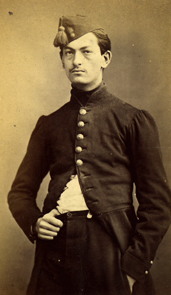
\includegraphics[width=\linewidth]{images/book3/b1-michel-levy.jpg}

{\scriptsize Michel-Lévy als student, rond 1862. Publiek domein.}
\end{minipage}
\end{history}

Twee golven die een korrel verlaten, kunnen een extra, bekende \omterm{def:b1:optical-mineralogy:retardation}{retardatie} krijgen door een hulpplaatje dat boven de doorsnede onder \ang{45} ten opzichte van de
polarisatoren wordt ingeschoven. Het meest voorkomende is gesneden om het \omterm{def:b1:optical-mineralogy:interference-colour}{eerste-orde} rood te tonen, een \omterm{def:b1:optical-mineralogy:retardation}{retardatie} van ongeveer \qty{540}{nm}. Als de langzame
trillingsrichting van de korrel evenwijdig is aan de langzame richting van het plaatje, tellen de vertragingen op en stijgt de kleur van de korrel met ongeveer
één \omterm{def:b1:optical-mineralogy:interference-colour}{orde}; is zij evenwijdig aan de snelle richting, dan trekken zij elkaar af en daalt de kleur. Een \omterm{def:b1:optical-mineralogy:interference-colour}{eerste-orde} grijze korrel van \qty{100}{nm} wordt \omterm{def:b1:optical-mineralogy:interference-colour}{tweede-orde}
blauw (\qty{640}{nm}) in de ene oriëntatie en \omterm{def:b1:optical-mineralogy:interference-colour}{eerste-orde} oranje (\qty{440}{nm}) in de andere; de test laat zien welke van de twee trillingsrichtingen van de korrel
de langzame is, een eigenschap die gebruikt wordt om langgerekte mineralen te identificeren.

\section{Mineralen herkennen in slijpplaat}

\begin{definition}[Tweeling, polysynthetische tweeling]\label{def:b1:optical-mineralogy:twin}
Een \emph{tweeling}\index{tweeling (kristal)} is een verwassing van twee of meer kristallen van hetzelfde \omterm{def:b1:rock-forming-minerals:mineral}{mineraal} waarvan de roosters verwant zijn door een symmetrie
die het kristal zelf niet heeft, zoals een spiegeling over een vlak (het tweelingvlak). \emph{Polysynthetische tweeling}\index{polysynthetische tweeling} is een herhaalde
tweeling op evenwijdige vlakken, die een kristal verdeelt in dunne evenwijdige lamellen waarvan de oriëntaties afwisselen.
\end{definition}

Tussen \omterm{def:b1:field-lab-methods-1:microscope}{gekruiste polarisatoren} doven de lamellen van een \omterm{def:b1:optical-mineralogy:twin}{polysynthetische tweeling} om en om uit: de helft ervan is donker wanneer de andere helft helder is, en het
kristal ziet er gestreept uit. \omterm{def:b1:rock-forming-minerals:groups}{Plagioklaas} toont bijna altijd deze strepen, die haar meteen van kwarts en van \omterm{def:b1:rock-forming-minerals:groups}{alkaliveldspaat} onderscheiden; haar andere kenmerk, laag
\omterm{def:b1:optical-mineralogy:relief}{reliëf} en \omterm{def:b1:optical-mineralogy:interference-colour}{eerste-orde} grijze tot witte kleuren, deelt zij met hen. De \omterm{def:b1:optical-mineralogy:extinction}{uitdovingshoeken} van de twee sets lamellen, aan weerszijden van het tweelingvlak gemeten, hangen
af van de samenstelling van de \omterm{def:b1:rock-forming-minerals:groups}{plagioklaas}, en diagrammen van die hoeken geven haar anortietgehalte.

\begin{method}[Een mineraal in slijpplaat identificeren]\label{met:b1:optical-mineralogy:identify}
\begin{enumerate}
  \item In \omterm{def:b1:field-lab-methods-1:microscope}{vlakgepolariseerd licht}: let op of de korrel ondoorzichtig is; haar kleur en \omterm{def:b1:optical-mineralogy:pleochroism}{pleochroïsme} (draai de tafel); haar \omterm{def:b1:optical-mineralogy:relief}{reliëf}, en aan welke kant van $1.54$
        haar index ligt (\omterm{def:b1:optical-mineralogy:relief}{Becke-lijn}); haar vorm en splijtingen, en de hoek tussen twee splijtingen.
  \item Tussen \omterm{def:b1:field-lab-methods-1:microscope}{gekruiste polarisatoren}: controleer of zij donker blijft (isotroop, of een doorsnede loodrecht op een \omterm{def:b1:optical-mineralogy:optic-axis}{optische as}); zoek onder de korrels van hetzelfde
        \omterm{def:b1:rock-forming-minerals:mineral}{mineraal} de hoogste \omterm{def:b1:optical-mineralogy:interference-colour}{interferentiekleur} en lees de \omterm{def:b1:optical-mineralogy:birefringence}{dubbelbreking} af op het \omterm{def:b1:optical-mineralogy:interference-colour}{Michel-Lévy-diagram} voor de dikte van de doorsnede.
  \item Meet de \omterm{def:b1:optical-mineralogy:extinction}{uitdovingshoek} op korrels die een splijting of een lengterichting tonen; zoek naar \omterm{def:b1:optical-mineralogy:twin}{tweelingvorming} (polysynthetische strepen, enkelvoudige \omterm{def:b1:optical-mineralogy:twin}{tweelingen}).
  \item Vergelijk met een tabel van optische eigenschappen (\cref{tab:b1:optical-mineralogy:key}) en met de mineralen die het gesteente kan bevatten
        (\cref{ch:b1:rock-forming-minerals}).
\end{enumerate}
\end{method}

\begin{table}[htbp]
\centering\footnotesize
\setlength{\tabcolsep}{3pt}
% ledger: hom:quartz-optics, hom:orthoclase-optics, hom:albite-optics, hom:anorthite-optics, hom:muscovite-optics, hom:biotite-optics, hom:hornblende-optics, hom:diopside-optics, hom:forsterite-optics, hom:fayalite-optics, hom:almandine-optics, hom:calcite-optics, hom:magnetite-optics
\begin{tabular}{@{}>{\raggedright\arraybackslash}p{2.0cm}>{\raggedright\arraybackslash}p{2.6cm}>{\raggedright\arraybackslash}p{2.3cm}>{\raggedright\arraybackslash}p{1.8cm}>{\raggedright\arraybackslash}p{3.0cm}>{\raggedright\arraybackslash}p{3.8cm}@{}}
\hline
\omterm{def:b1:rock-forming-minerals:mineral}{mineraal} & kleur (PPL) & indices & dub\-bel\-breking & hoogste kleur bij \qty{30}{\micro m} & overige kenmerken \\
\hline
kwarts & kleurloos & 1.544--1.553 & 0.009 & \omterm{def:b1:optical-mineralogy:interference-colour}{eerste-orde} wit & geen splijting; geen \omterm{def:b1:optical-mineralogy:twin}{tweelingen} zichtbaar; \omterm{def:b1:optical-mineralogy:optic-axis}{eenassig} \\
ortoklaas & kleurloos, vaak troebel & 1.518--1.525 & 0.005 & \omterm{def:b1:optical-mineralogy:interference-colour}{eerste-orde} grijs & negatief \omterm{def:b1:optical-mineralogy:relief}{reliëf}; enkelvoudige \omterm{def:b1:optical-mineralogy:twin}{tweelingen} \\
\omterm{def:b1:rock-forming-minerals:groups}{plagioklaas} & kleurloos & 1.526--1.590 & 0.008--0.013 & \omterm{def:b1:optical-mineralogy:interference-colour}{eerste-orde} wit tot lichtgeel & polysynthetische \omterm{def:b1:optical-mineralogy:twin}{tweelingvorming} \\
muscoviet & kleurloos & 1.552--1.618 & 0.035--0.042 & helder tweede- tot \omterm{def:b1:optical-mineralogy:interference-colour}{derde-orde} & één volmaakte splijting; rechte uitdoving \\
biotiet & bruin, groen & 1.565--1.696 & 0.04--0.07 & verborgen door de eigen kleur & sterk \omterm{def:b1:optical-mineralogy:pleochroism}{pleochroïsch}; één volmaakte splijting \\
hoornblende & groen, bruin & 1.675--1.695 & 0.020 & \omterm{def:b1:optical-mineralogy:interference-colour}{tweede-orde} blauw & \omterm{def:b1:optical-mineralogy:pleochroism}{pleochroïsch}; splijtingen bij \ang{56}/\ang{124}; uitdoving \ang{15}--\ang{19} \\
diopsied & kleurloos & 1.664--1.694 & 0.030 & \omterm{def:b1:optical-mineralogy:interference-colour}{tweede-orde} geel & splijtingen bij ongeveer \ang{87}/\ang{93}; uitdoving ongeveer \ang{38} \\
\omterm{def:b1:rock-forming-minerals:groups}{olivijn} & kleurloos (Mg) tot lichtgeel (Fe) & 1.635--1.879 & 0.035--0.052 & einde van tweede tot derde \omterm{def:b1:optical-mineralogy:interference-colour}{orde} & hoog \omterm{def:b1:optical-mineralogy:relief}{reliëf}; onregelmatige scheuren, geen goede splijting \\
\omterm{def:b1:rock-forming-minerals:groups}{granaat} & kleurloos tot lichtroze & 1.830 (almandien) & isotroop & zwart & zeer hoog \omterm{def:b1:optical-mineralogy:relief}{reliëf}; zes- of achtzijdige omtrekken \\
calciet & kleurloos & 1.486--1.658 & 0.172 & \omterm{def:b1:optical-mineralogy:interference-colour}{hoogste-orde} wit & \omterm{def:b1:optical-mineralogy:relief}{reliëf} verandert bij draaien; romboëdrische splijting \\
magnetiet & ondoorzichtig & --- & --- & --- & zwart in beide lichten \\
\hline
\end{tabular}
\caption{Optische eigenschappen van veelvoorkomende gesteentevormende mineralen in \omterm{def:b1:field-lab-methods-1:thin-section}{slijpplaat}.
PPL: \omterm{def:b1:field-lab-methods-1:microscope}{vlakgepolariseerd licht}. De hoogste kleur wordt afgelezen op het \omterm{def:b1:optical-mineralogy:interference-colour}{Michel-Lévy-diagram} bij
$\Delta = \qty{30000}{nm}\times\delta$.}
\label{tab:b1:optical-mineralogy:key}
\end{table}

\begin{omfigure}
\setlength{\tabcolsep}{2pt}
\begin{tabular}{cc}
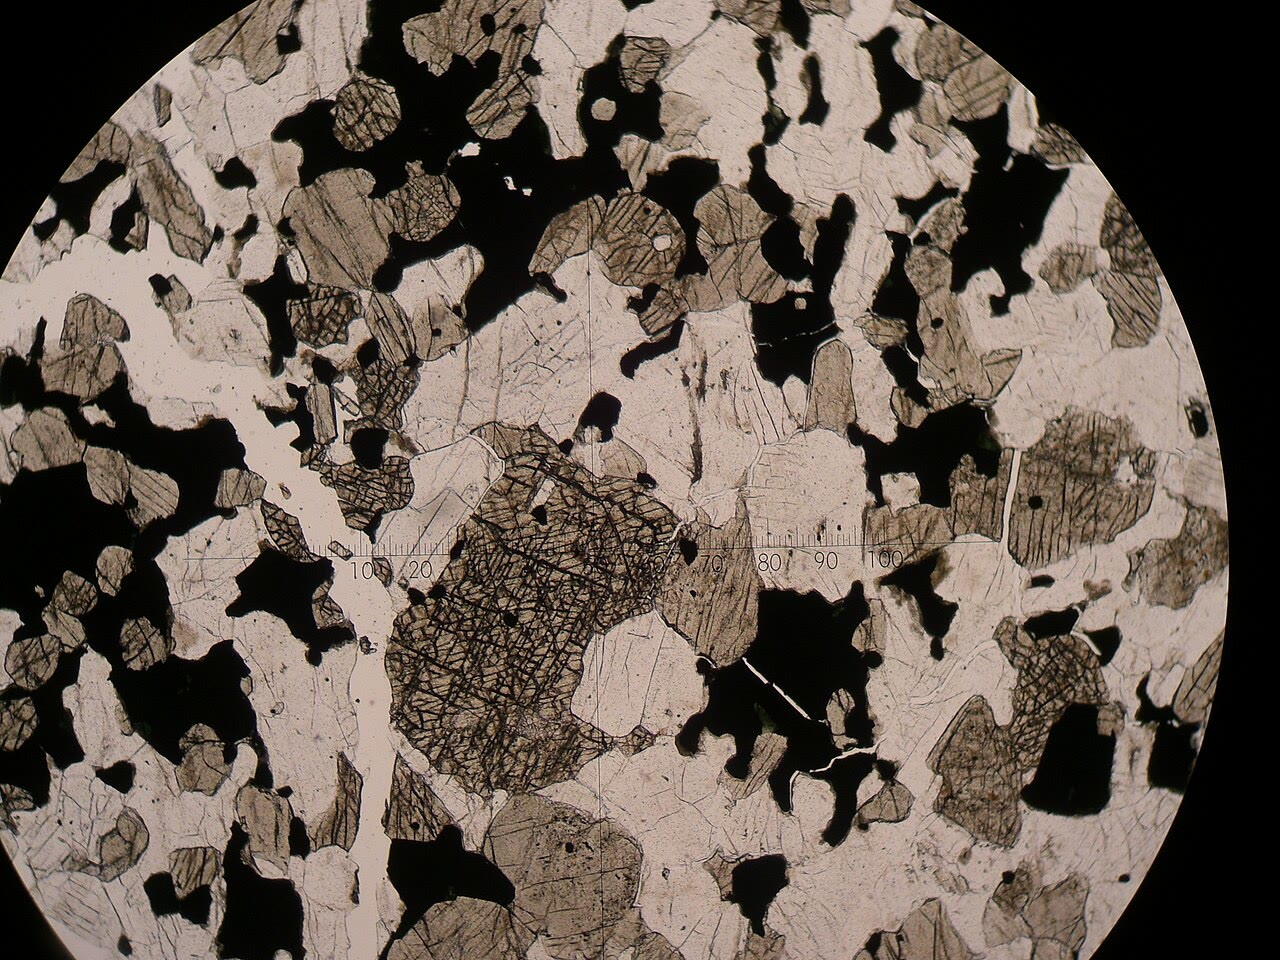
\includegraphics[width=0.485\linewidth]{images/book3/b1-gabbro-ppl.jpg} &
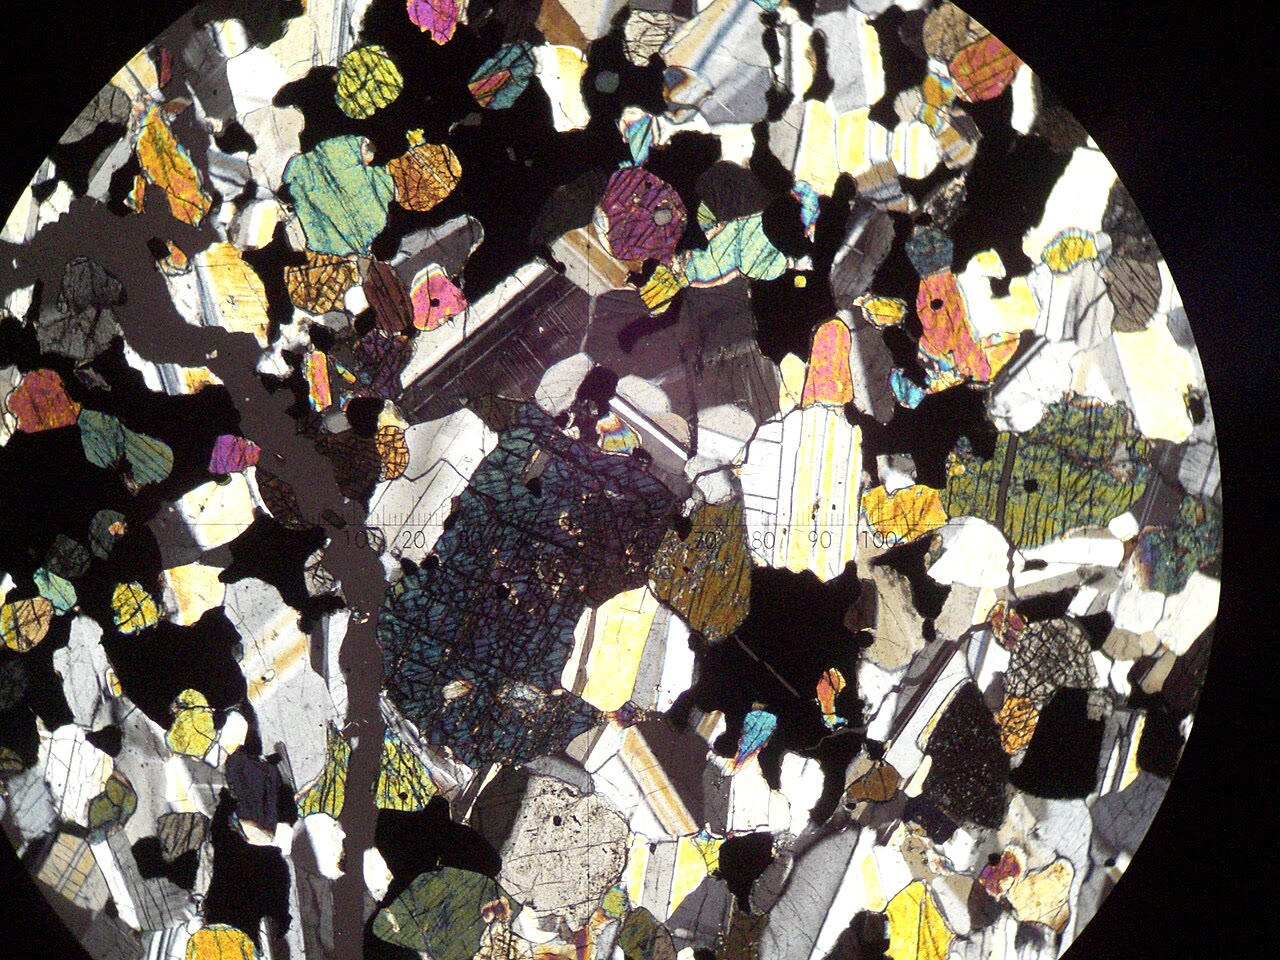
\includegraphics[width=0.485\linewidth]{images/book3/b1-gabbro-xpl.jpg} \\
{\small (a) \omterm{def:b1:field-lab-methods-1:microscope}{vlakgepolariseerd licht}} & {\small (b) \omterm{def:b1:field-lab-methods-1:microscope}{gekruiste polarisatoren}} \\
\end{tabular}
% ledger: commons:gabbro-ppl, commons:gabbro-xpl

\medskip
{\small Hetzelfde veld van een gabbro in \omterm{def:b1:field-lab-methods-1:thin-section}{slijpplaat}. In \omterm{def:b1:field-lab-methods-1:microscope}{vlakgepolariseerd licht} (a) is \omterm{def:b1:rock-forming-minerals:groups}{plagioklaas} kleurloos met laag \omterm{def:b1:optical-mineralogy:relief}{reliëf}, zijn de pyroxeen- en olivijnkorrels
bleek bruingrijs met hoog \omterm{def:b1:optical-mineralogy:relief}{reliëf} en dichte scheuren, en is het opake erts zwart; de schaal is een micrometer in het oculair. Tussen \omterm{def:b1:field-lab-methods-1:microscope}{gekruiste polarisatoren} (b) zijn de
plagioklaaslatten gestreept door polysynthetische \omterm{def:b1:optical-mineralogy:twin}{tweelingvorming}, stralen de pyroxeen- en olivijnkorrels in \omterm{def:b1:optical-mineralogy:interference-colour}{tweede-orde} kleuren, en blijft het erts zwart. Foto's
Chmee2, CC BY-SA 3.0 (Wikimedia Commons).}
\end{omfigure}

\begin{inthelab}[Een sessie bij de microscoop]
\begin{minipage}[t]{0.55\linewidth}\vspace{0pt}
Een petroloog die een nieuwe \omterm{def:b1:field-lab-methods-1:thin-section}{slijpplaat} beschrijft, werkt haar eerst bij lage vergroting door, om de textuur en de hoofdmineralen te zien, en dan korrel
voor korrel. Voor elk \omterm{def:b1:rock-forming-minerals:mineral}{mineraal} noteert zij de waarnemingen van de methode hierboven, schat zij het aandeel ervan in het veld, en let zij op hoe de korrels elkaar raken:
welke eerst kristalliseerden, welke de ruimten vullen die overblijven, welke andere vervangen. Lichtmetingen worden gedaan met de tafel die in graden is geijkt en een
hulpplaatje; samenstellingen, wanneer die ertoe doen, worden later met een microsonde op dezelfde doorsnede gemeten. Een onderwijslaboratorium werkt op dezelfde manier,
met één microscoop per student en een doos referentiedoorsneden van bekende mineralen ernaast.
\end{minipage}\hfill
\begin{minipage}[t]{0.42\linewidth}\vspace{0pt}
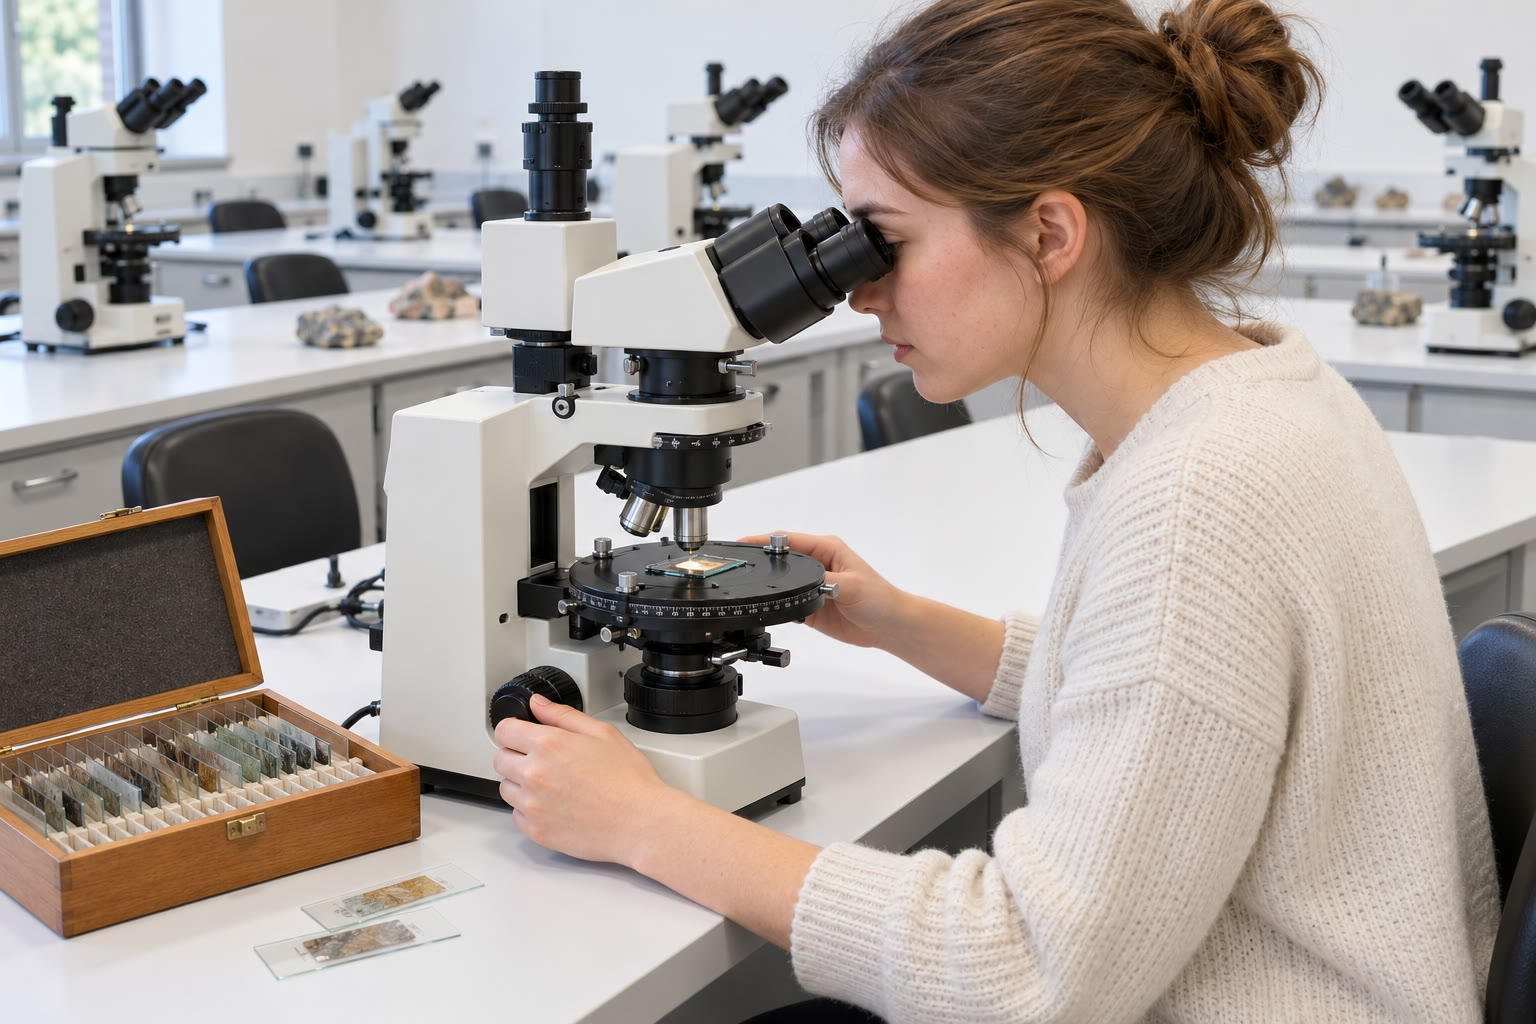
\includegraphics[width=\linewidth]{images/book3/ai/b1-microscope-student.jpg}

{\scriptsize Een student bij een \omterm{def:b1:field-lab-methods-1:microscope}{polariserende microscoop} in een onderwijslaboratorium
(AI-gegenereerde illustratie).}
\end{minipage}
\end{inthelab}

\section{Oefeningen}

\begin{exercise}[$\star$]\label{exo:b1:optical-mineralogy:1}
Bereken de grootste \omterm{def:b1:optical-mineralogy:retardation}{retardatie} van kwarts ($\delta = 0.009$) en van calciet ($\delta = 0.172$) in een doorsnede van \qty{30}{\micro m} dik. Beschrijf met het
\omterm{def:b1:optical-mineralogy:interference-colour}{Michel-Lévy-diagram} de kleur van elk.
% ledger: hom:quartz-optics, hom:calcite-optics
\end{exercise}

\begin{exercise}[$\star$]\label{exo:b1:optical-mineralogy:2}
Een korrel wordt op de tafel gedraaid tussen \omterm{def:b1:field-lab-methods-1:microscope}{gekruiste polarisatoren}. Bereken $I/I_0$, als breuk van haar maximum, bij $\theta = 0$, \ang{22.5}, \ang{45}, \ang{67.5} en
\ang{90} van een \omterm{def:b1:optical-mineralogy:extinction}{uitdovingsstand}.
\end{exercise}

\begin{exercise}[$\star$]\label{exo:b1:optical-mineralogy:3}
Leg uit waarom een \omterm{def:b1:rock-forming-minerals:groups}{granaat} tussen \omterm{def:b1:field-lab-methods-1:microscope}{gekruiste polarisatoren} in elke stand van de tafel zwart blijft, en waarom een kwartskorrel dat ook kan doen. Hoe zou men ze in
\omterm{def:b1:field-lab-methods-1:microscope}{vlakgepolariseerd licht} onderscheiden?
\end{exercise}

\begin{exercise}[$\star$]\label{exo:b1:optical-mineralogy:4}
Rangschik naar \omterm{def:b1:optical-mineralogy:relief}{reliëf}, in een middel met index $1.54$, ortoklaas ($n$ ongeveer $1.52$), kwarts ($1.55$), forsteriet ($1.65$) en almandien ($1.83$). Welke heeft negatief
\omterm{def:b1:optical-mineralogy:relief}{reliëf}? In welke richting beweegt haar \omterm{def:b1:optical-mineralogy:relief}{Becke-lijn} wanneer de scherpstelling wordt verhoogd?
% ledger: hom:orthoclase-optics, hom:quartz-optics, hom:forsterite-optics, hom:almandine-optics
\end{exercise}

\begin{exercise}[$\star\star$]\label{exo:b1:optical-mineralogy:5}
In een \omterm{def:b1:field-lab-methods-1:thin-section}{slijpplaat} van \qty{30}{\micro m} tonen de korrels van een groen \omterm{def:b1:optical-mineralogy:pleochroism}{pleochroïsch} \omterm{def:b1:rock-forming-minerals:mineral}{mineraal} met twee splijtingen bij \ang{56} en \ang{124} hoogstens een \omterm{def:b1:optical-mineralogy:interference-colour}{tweede-orde}
blauw, op het diagram afgelezen als $\Delta = \qty{650}{nm}$. Bereken zijn \omterm{def:b1:optical-mineralogy:birefringence}{dubbelbreking} en noem het \omterm{def:b1:rock-forming-minerals:mineral}{mineraal} met \cref{tab:b1:optical-mineralogy:key}.
\end{exercise}

\begin{exercise}[$\star\star$]\label{exo:b1:optical-mineralogy:6}
Gebruik \cref{prop:b1:optical-mineralogy:relief} met $n_m = 1.54$ en $i = \ang{30}$, en bereken de afbuiging aan de rand van een kwartskorrel ($n = 1.553$) en van een
forsterietkorrel ($n = 1.651$), in graden, en de verhouding van de twee. Controleer de tweede exact met de wet van Snellius.
\end{exercise}

\begin{exercise}[$\star\star$]\label{exo:b1:optical-mineralogy:7}
Een \omterm{def:b1:optical-mineralogy:interference-colour}{eerste-orde} rood plaatje heeft $\Delta = \qty{540}{nm}$. Een kwartskorrel van $\Delta = \qty{270}{nm}$ wordt op \ang{45} geplaatst met het plaatje ingeschoven. Wat zijn
de twee mogelijke totale \omterm{def:b1:optical-mineralogy:retardation}{retardaties}, en welke kleuren geven zij op het diagram? Welke oriëntatie brengt de twee langzame richtingen evenwijdig?
\end{exercise}

\begin{exercise}[$\star\star$]\label{exo:b1:optical-mineralogy:8}
Op zijn taps toelopende rand dunt een korrel fayaliet ($\delta = 0.052$) van \qty{30}{\micro m} tot nul af. Hoeveel rood-violette tinten, die de \omterm{def:b1:optical-mineralogy:interference-colour}{ordes} beëindigen bij
542, 1074 en \qty{1605}{nm}, verschijnen als gekleurde randen tussen de rand en het deel van de korrel met volledige dikte?
% ledger: hom:fayalite-optics
\end{exercise}

\begin{exercise}[$\star\star$]\label{exo:b1:optical-mineralogy:9}
Op verschillende langgerekte korrels met één goede splijting meet een geoloog \omterm{def:b1:optical-mineralogy:extinction}{uitdovingshoeken} van \ang{0}, \ang{21}, \ang{36} en \ang{37} tussen het splijtspoor en de
langzame trillingsrichting. Waarom verschillen de waarden? Is het \omterm{def:b1:rock-forming-minerals:mineral}{mineraal} waarschijnlijker diopsied of hoornblende?
% ledger: hom:diopside-optics, hom:hornblende-optics
\end{exercise}

\begin{exercise}[$\star\star\star$]\label{exo:b1:optical-mineralogy:10}
Doe het bewijs van \cref{thm:b1:optical-mineralogy:intensity} opnieuw met de analysator evenwijdig aan de polarisator, en toon aan dat
$I_\parallel = I_0\bigl(1 - \sin^2 2\theta\sin^2(\pi\Delta/\lambda)\bigr)$. Welke kleur toont een korrel van $\Delta = \qty{550}{nm}$ op \ang{45} tussen evenwijdige polarisatoren?
\end{exercise}

\begin{exercise}[$\star\star\star$]\label{exo:b1:optical-mineralogy:11}
Voor een calcietkorrel met $\Delta = \qty{5000}{nm}$ verdwijnt de factor $\sin^2(\pi\Delta/\lambda)$ wanneer $\Delta/\lambda$ een geheel getal is. (a) Hoe vaak verdwijnt zij
tussen \num{400} en \qty{700}{nm}? (b) Toon aan dat dicht bij $\lambda = \qty{550}{nm}$ twee opeenvolgende nullen ongeveer $\lambda^2/\Delta$ uit elkaar liggen, en bereken dat.
(c) Leg uit waarom de korrel bijna wit lijkt.
\end{exercise}

\begin{exercise}[$\star\star\star$]\label{exo:b1:optical-mineralogy:12}
Toon aan dat een korrel tussen \omterm{def:b1:field-lab-methods-1:microscope}{gekruiste polarisatoren}, gemiddeld over een volledige omwenteling van de tafel, $\frac12 I_0\sin^2(\pi\Delta/\lambda)$ doorlaat. Een geoloog
schat \omterm{def:b1:optical-mineralogy:birefringence}{dubbelbreking} uit de hoogste kleur van elk \omterm{def:b1:rock-forming-minerals:mineral}{mineraal}, uitgaande van \qty{30}{\micro m}, in een doorsnede die in werkelijkheid \qty{25}{\micro m} dik is. Met welke factor
zijn al haar waarden fout, en in welke richting?
\end{exercise}

\section{Probleem: De mineralen van een onbekende slijpplaat identificeren}

\begin{problem}[{Weekendprobleem --- reliëf, pleochroïsme en interferentiekleuren waarnemen, de dikte van een doorsnede
met kwarts meten en haar mineralen benoemen}]
\label{pb:b1:optical-mineralogy:1}
% values: calc/ch08.py; optical data: ledger hom:*-optics
% ledger: hom:quartz-optics, hom:diopside-optics, hom:forsterite-optics, hom:albite-optics, hom:anorthite-optics, hom:hornblende-optics, hom:biotite-optics
Een \omterm{def:b1:field-lab-methods-1:thin-section}{slijpplaat} van een onbekend stollingsgesteente, gemonteerd in een hars met index $1.540$, wordt gezegd \qty{30}{\micro m} dik te zijn.
Zij bevat vijf mineralen, aangeduid met A tot E. Gebruik de tabel van optische eigenschappen van het hoofdstuk, het \omterm{def:b1:optical-mineralogy:interference-colour}{Michel-Lévy-diagram} en de
volgende waarden: kwarts $n_\omega = 1.544$, $n_\varepsilon = 1.553$; diopsied $n_\alpha = 1.664$, $n_\beta = 1.672$, $n_\gamma = 1.694$.

\medskip
\noindent\textbf{Deel I --- Vlakgepolariseerd licht.}
\begin{enumerate}
  \item \omterm{def:b1:rock-forming-minerals:mineral}{Mineraal} A is kleurloos, met korrelgrenzen die moeilijk te zien zijn. \omterm{def:b1:rock-forming-minerals:mineral}{Mineraal} B is kleurloos, met sterke donkere randen en
        twee splijtingen die bij ongeveer \ang{87} samenkomen. Welke heeft het hoogste \omterm{def:b1:optical-mineralogy:relief}{reliëf}?
  \item Neem A als kwarts en B als diopsied, en bereken $|n - n_m|$ met het gemiddelde van de hoofdindices van elk.
  \item Gebruik \cref{prop:b1:optical-mineralogy:relief} en bereken de verhouding van de afbuigingen aan hun randen bij
        dezelfde helling van de grens.
  \item Bij het scherpstellen beweegt de \omterm{def:b1:optical-mineralogy:relief}{Becke-lijn} van B de korrel in. Wat toont dit?
  \item \omterm{def:b1:rock-forming-minerals:mineral}{Mineraal} C draait van lichtgeel naar donkerbruin wanneer de tafel draait, het donkerst wanneer zijn enkele splijting langs
        de polarisator ligt. Noem de eigenschap en het \omterm{def:b1:rock-forming-minerals:mineral}{mineraal}.
  \item \omterm{def:b1:rock-forming-minerals:mineral}{Mineraal} D is kleurloos, van laag \omterm{def:b1:optical-mineralogy:relief}{reliëf}, in lange latten; E is groen tot geel en \omterm{def:b1:optical-mineralogy:pleochroism}{pleochroïsch}, met twee splijtingen bij
        \ang{124}. Wat suggereert de hoek voor E?
\end{enumerate}

\medskip
\noindent\textbf{Deel II --- De dikte van de doorsnede.}
\begin{enumerate}[resume]
  \item Wat is de grootste \omterm{def:b1:optical-mineralogy:retardation}{retardatie} van kwarts in een doorsnede van precies \qty{30}{\micro m}? Welke kleur heeft zij?
  \item Waarom moet de grootste \omterm{def:b1:optical-mineralogy:retardation}{retardatie} worden gezocht onder vele korrels van A, en niet op één van hen worden gemeten?
  \item De hoogste kleur die de korrels van A tonen is een \omterm{def:b1:optical-mineralogy:interference-colour}{eerste-orde} bleekgeel; een kwarts-wigvergelijker geeft hun \omterm{def:b1:optical-mineralogy:retardation}{retardatie} als
        \qty{342}{nm}. Bereken de werkelijke dikte van de doorsnede.
  \item Met hoeveel procent is de doorsnede dikker dan zij zou moeten zijn?
  \item Bereken bij $\lambda = \qty{550}{nm}$ en \ang{45} van de uitdoving $I/I_0$ voor deze kwartskorrel, en voor dezelfde korrel in een
        doorsnede van \qty{30}{\micro m}.
  \item Bereken het bereik van de \omterm{def:b1:optical-mineralogy:retardation}{retardaties} van D, aangenomen als \omterm{def:b1:rock-forming-minerals:groups}{plagioklaas} ($\delta = 0.008$ tot $0.013$), in deze doorsnede,
        en zeg of haar kleuren in de eerste \omterm{def:b1:optical-mineralogy:interference-colour}{orde} blijven.
\end{enumerate}

\medskip
\noindent\textbf{Deel III --- De dubbelbreking van B.}
\begin{enumerate}[resume]
  \item De hoogste kleur van B is een blauw dat als $\Delta = \qty{1140}{nm}$ wordt afgelezen. In welke \omterm{def:b1:optical-mineralogy:interference-colour}{orde} ligt zij?
  \item Bereken de \omterm{def:b1:optical-mineralogy:birefringence}{dubbelbreking} van B met de dikte die in vraag 9 is gevonden.
  \item Welke \omterm{def:b1:optical-mineralogy:birefringence}{dubbelbreking} zou men hebben gevonden als men \qty{30}{\micro m} had aangenomen? Welk kleurloos \omterm{def:b1:rock-forming-minerals:mineral}{mineraal} van hoog
        \omterm{def:b1:optical-mineralogy:relief}{reliëf} zou dat hebben gesuggereerd, en waarom past het niet in een gesteente met kwarts (overweeg
        \ce{Mg2SiO4 + SiO2 -> 2 MgSiO3})?
  \item Vergelijk het resultaat van vraag 14 met de tabel, samen met het \omterm{def:b1:optical-mineralogy:relief}{reliëf} en de splijtingen van B, en trek een conclusie.
  \item Welke kleur zou B hoogstens tonen in een correcte doorsnede van \qty{30}{\micro m}?
  \item De doorsnede wordt tot \qty{30}{\micro m} afgeslepen. Met hoeveel moet zij dunner worden, en wat is dan de hoogste kleur van kwarts?
\end{enumerate}

\medskip
\noindent\textbf{Deel IV --- Uitdoving en tweelingvorming.}
\begin{enumerate}[resume]
  \item De latten van D zijn verdeeld in evenwijdige strepen die om en om doven. Noem het kenmerk en het \omterm{def:b1:rock-forming-minerals:mineral}{mineraal}.
  \item De strepen van één latt doven uit bij \ang{27} en \ang{28} aan weerszijden van het tweelingvlak. Wat geven zulke hoeken,
        op veel latten gemeten, wanneer zij met gepubliceerde diagrammen worden vergeleken?
  \item De grootste \omterm{def:b1:optical-mineralogy:extinction}{uitdovingshoek} tussen de splijtingen van E en zijn langzame richting is \ang{17}. Noem E.
  \item Bereken de grootste \omterm{def:b1:optical-mineralogy:retardation}{retardatie} van E in deze doorsnede en de kleur die zij toont.
  \item Een korrel van B blijft tijdens een volledige omwenteling donker. Leg uit hoe het hetzelfde \omterm{def:b1:rock-forming-minerals:mineral}{mineraal} kan zijn als de heldere
        korrels van B.
  \item Noem de mineralen A tot E, en zeg wat voor gesteente zij vormen.
  \item Wat is de werkelijke dikte van de doorsnede, in micrometer?
\end{enumerate}
\end{problem}
